%==============================================================================
%== template for LATEX poster =================================================
%==============================================================================
%
%--A0 beamer slide-------------------------------------------------------------
\documentclass[final]{beamer}\usepackage[]{graphicx}\usepackage[]{color}
%% maxwidth is the original width if it is less than linewidth
%% otherwise use linewidth (to make sure the graphics do not exceed the margin)
\makeatletter
\def\maxwidth{ %
  \ifdim\Gin@nat@width>\linewidth
    \linewidth
  \else
    \Gin@nat@width
  \fi
}
\makeatother

\definecolor{fgcolor}{rgb}{0.345, 0.345, 0.345}
\newcommand{\hlnum}[1]{\textcolor[rgb]{0.686,0.059,0.569}{#1}}%
\newcommand{\hlstr}[1]{\textcolor[rgb]{0.192,0.494,0.8}{#1}}%
\newcommand{\hlcom}[1]{\textcolor[rgb]{0.678,0.584,0.686}{\textit{#1}}}%
\newcommand{\hlopt}[1]{\textcolor[rgb]{0,0,0}{#1}}%
\newcommand{\hlstd}[1]{\textcolor[rgb]{0.345,0.345,0.345}{#1}}%
\newcommand{\hlkwa}[1]{\textcolor[rgb]{0.161,0.373,0.58}{\textbf{#1}}}%
\newcommand{\hlkwb}[1]{\textcolor[rgb]{0.69,0.353,0.396}{#1}}%
\newcommand{\hlkwc}[1]{\textcolor[rgb]{0.333,0.667,0.333}{#1}}%
\newcommand{\hlkwd}[1]{\textcolor[rgb]{0.737,0.353,0.396}{\textbf{#1}}}%

\usepackage{framed}
\makeatletter
\newenvironment{kframe}{%
 \def\at@end@of@kframe{}%
 \ifinner\ifhmode%
  \def\at@end@of@kframe{\end{minipage}}%
  \begin{minipage}{\columnwidth}%
 \fi\fi%
 \def\FrameCommand##1{\hskip\@totalleftmargin \hskip-\fboxsep
 \colorbox{shadecolor}{##1}\hskip-\fboxsep
     % There is no \\@totalrightmargin, so:
     \hskip-\linewidth \hskip-\@totalleftmargin \hskip\columnwidth}%
 \MakeFramed {\advance\hsize-\width
   \@totalleftmargin\z@ \linewidth\hsize
   \@setminipage}}%
 {\par\unskip\endMakeFramed%
 \at@end@of@kframe}
\makeatother

\definecolor{shadecolor}{rgb}{.97, .97, .97}
\definecolor{messagecolor}{rgb}{0, 0, 0}
\definecolor{warningcolor}{rgb}{1, 0, 1}
\definecolor{errorcolor}{rgb}{1, 0, 0}
\newenvironment{knitrout}{}{} % an empty environment to be redefined in TeX

\usepackage{alltt}
\usepackage{graphicx, color}
%% maxwidth is the original width if it is less than linewidth
%% otherwise use linewidth (to make sure the graphics do not exceed the margin)
\makeatletter
\def\maxwidth{ %
  \ifdim\Gin@nat@width>\linewidth
    \linewidth
  \else
    \Gin@nat@width
  \fi
}
\makeatother

\usepackage[
  natbib = true,
    backend=bibtex,
    isbn=false,
    url=false,
    doi=false,
    eprint=false,
]{biblatex}
%{\tiny
\bibliography{../CT_Pipeline_l}
%}
\renewcommand*{\bibfont}{\scriptsize}


\graphicspath{{../maps/}{../}}


\def\newblock{\hskip .11em plus .33em minus .07em} %for natbib and beamer 
\usepackage[orientation=landscape,size=a0,
            scale=1,         % font scale factor
            size=custom,width=140,height=90,
           ]{beamerposter}
\setbeamertemplate{frametitle}{
    \vspace{-5cm}\\
    \insertframetitle
}         
           
\geometry{
  hmargin=2.5cm, % little modification of margins
  vmargin = 0cm,
  head=0cm  
}

%
%\usepackage{floatrow}
\usepackage{float}
%\usepackage{subfigure}
\usepackage{caption}
\captionsetup{compatibility=false}
\usepackage{subcaption}


\usepackage[utf8]{inputenc}
%\usepackage{verbatim}

\linespread{1.15}
%
%==The poster style============================================================
\usetheme{sharelatex}

%==Title, date and authors of the poster=======================================
\title
%[Super Conference, 1 - 10 July 2013, New York, USA] % Conference
{ % Poster title
Intracranial hemorrhage localization: A CT imaging pipeline
}





%\author{ % Authors
%John Muschelli\inst{1}, Elizabeth Sweeney\inst{1}, Ciprian Crainiceanu\inst{1}
%}
%\institute
%[Johns Hopkins Bloomberg School of Public Health] % General University
%{
%\inst{1} Johns Hopkins Bloomberg School of Public Health
%}
\author{ % Authors
John Muschelli$^{1}$, Natalie L. Ullman$^{2}$, Elizabeth M. Sweeney$^{1}$, Ani Eloyan$^{1}$, Ciprian M. Crainiceanu$^{1}$, Daniel F. Hanley$^{2}$
}

\institute
[Johns Hopkins Bloomberg School of Public Health] % General University
{
%Johns Hopkins Bloomberg School of Public Health
\bf{1} Department of Biostatistics, Bloomberg School of Public Health, Johns Hopkins University, Baltimore, MD, USA \\
\bf{2} Department of Neurology, Division of Brain Injury Outcomes,  Johns Hopkins Medical Institutions, Baltimore, MD, USA
}
\date{\today}


\usepackage{hyperref}
\IfFileExists{upquote.sty}{\usepackage{upquote}}{}
\IfFileExists{upquote.sty}{\usepackage{upquote}}{}

\begin{document}

\vspace{-3.5cm}
\newcommand{\stickynote}{
\includegraphics[height=1.5em]{blank_sticky_note.png}\;}

\begin{frame}[fragile]
\vspace{-3.5cm}
%==============================================================================
\begin{multicols}{2}
%==============================================================================
%==The poster content==========================================================
%==============================================================================
\section{Introduction: Intracranial Hemorrhage affects are elderly}

%Demog table
%reg - no ss
%3D HIst
%voxelwise
%Patient-level
%table

%\begin{minipage}[b]{.8\linewidth}
\vspace*{-0.5cm}
%\subsection{Strokes kill people}


%ICH is a a {\bf killer}: $\approx$10-15\% of all strokes and causes $\approx$30,000 annual deaths \citep{qureshi_spontaneous_2001}.  \\

%\subsection{}

Intracerebral hemorrhage (ICH) is a form of stroke where a blood vessel ruptures in the brain.\\

In 2009, $66\%$ of people hospitalized for stroke were  $\geq 65$ \cite{hall_hospitalization_2012}.  For every $10$ years over $55$ years of age, the risk of stroke doubles \cite{wolf_secular_1992, brown_stroke_1996}.  For adults over age $65$, the risk of dying from stroke is estimated to be $3$ to $7$ times that of the population \cite{feldmann_intracerebral_1994, di_carlo_stroke_2003}. 

%\subsection{How do we assess stroke?}
%
%The National Institutes of Health Stroke Scale (NIHSS) \citep{brott_measurements_1989} measures how severe a stroke is.  
%
%Computed tomography (CT) scans are taken and are the {\bf most commonly used diagnostic tool} in patients with ICH \citep{sahni_management_2007}. See Figure~\ref{f:reg}\protect\subref{reg:nat2}. \\
%
%Expert readers segment the ICH on the CT scan ``by hand'' using the DICOM tool OsiriX (OsiriX v. 4.1, Pixmeo; Geneva, Switzerland).


%%    \includegraphics[width=7in, height=5in]{./figure/lightbox.png}
%  \end{minipage}\hfill  
%  \begin{minipage}[b]{.2\linewidth}
%
%\raisebox{2em}{
%
\includegraphics[width=.8\linewidth]{man-drawing-brain.png}
%}
%{\scriptsize Images from \url{http://www.clker.com/clipart-outline-of-brain.html} and \url{http://www.clker.com/clipart-man-drawing.html}
%}

%\end{minipage}

\section{Goals and Demographics}

\begin{minipage}{\linewidth}
\begin{multicols}{2}


\begin{itemize}
\item Register patient CT scans to a common CT template
\item Create a 3D density map of where ICH occurring in a population of patients 
\item Determine if differences in ICH location relate to the NIHSS score (voxel-wise)
\item Generate a stroke region of interest (ROI) and associate it with health effects (NIHSS score)
\end{itemize}

This analysis included $111$ patients from the MISTIE ($N = 94$) and ICES ($N = 17$) trials.  In these trials, patients were randomized to standard of care medical management or an intervention.  Patients were required to have a pre-randomization scan with ICH segmentations. 

%\subsection{Demographics and Reader-Assessed ICH Locations} 

%\section{Study Population}

\vfill
\columnbreak

%The intervention involves drilling a hole in a patient's brain and sticking a catheter to deliver a rtPA, a clot buster (MISTIE) or sticking a endoscope and using suction to remove hemorrhage (ICES).  


% latex table generated in R 3.1.0 by xtable 1.7-3 package
% Wed Jul 23 12:03:50 2014
\begin{table}[ht]
\centering
\begin{tabular}{lc}
  \hline {\bf Variable (N = 111)} & {\bf N (\%) or Mean (SD)} \\ 
  \hline
Age in Years: Mean (SD) & 60.8 (11.2) \\ 
   \hline
NIHSS Score: Mean (SD) & 22.1 (8.7) \\ 
   \hline
Reader-Classified ICH Location &  \\ 
   \hline
\text{  } Putamen & 68 (61.3\%) \\ 
   \hline
\text{  } Lobar & 33 (29.7\%) \\ 
   \hline
\text{  } Globus Palidus & 6 (5.4\%) \\ 
   \hline
\text{  } Thalamus & 4 (3.6\%) \\ 
   \hline
\end{tabular}
\caption{Descriptive statistics of the demographic information on the patients.} 
\label{t:dem}
\end{table}


\end{multicols}
\end{minipage}

\section{Image Processing} 

\begin{figure}[htbp]
 \begin{subfigure}[t]{0.25\linewidth} 
  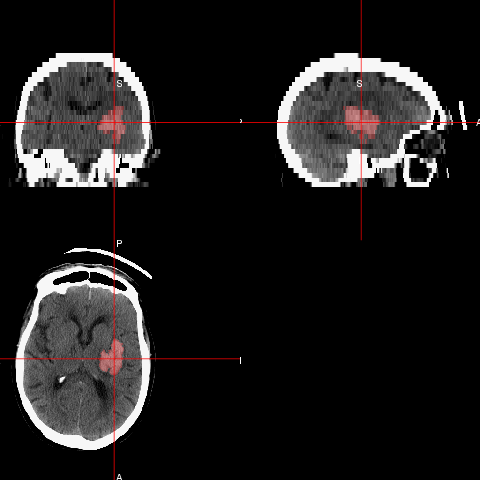
\includegraphics[width=\linewidth]{native_191-375_20100410_0404_CT_2_CT_STANDARD.png}
  \caption{\textbf{Original image} in native space}
 \label{reg:nat2}
  \end{subfigure}
 \begin{subfigure}[t]{0.25\linewidth} 
  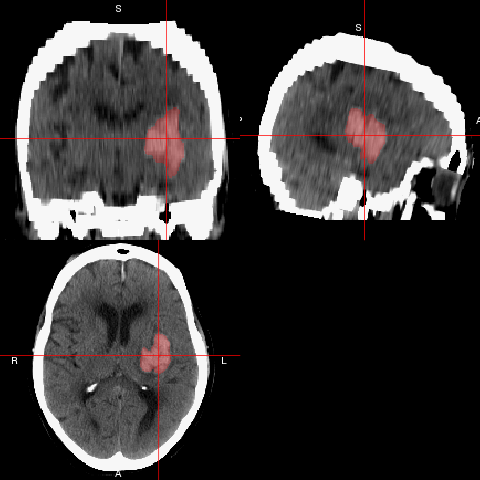
\includegraphics[width=\linewidth]{raw_spm_191-375_20100410_0404_CT_2_CT_STANDARD.png}
  \caption{\textbf{Registered image} with ICH mask highlighted in pink.}
  \label{reg:co2}
  \end{subfigure}
 \begin{subfigure}[t]{0.25\linewidth} 
  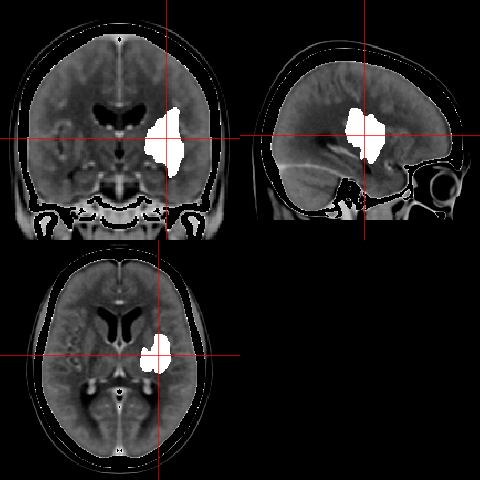
\includegraphics[width=\linewidth]{roi_spm_191-375_20100410_0404_CT_2_CT_STANDARD.png}
  \caption{\textbf{Template brain} with ICH mask overlaid.}
  \label{reg:temp2}
  \end{subfigure}
   \begin{minipage}[b]{0.2\linewidth}
	  	\caption{Patient brains were registered to the template using the Clinical toolbox \citep{rorden_age-specific_2012}, using SPM8's unified normalization–segmentation \citep{ashburner_unified_2005}. After registration, patient images are in the same space; information can be summarized spatially across patients. \vspace{1cm} \\
	  	{\bf Take Home Message: We can register people's brains to a template brain to compare across subjects.}
		}
	  \label{f:reg}
\end{minipage}  
%    \hfill
\end{figure}


\section{Voxel-wise Regression on NIHSS Score}


\begin{minipage}{.4\linewidth}
	We did voxel-wise linear regressions on the NIHSS score for voxels that had $> 10$ patients with ICH at that location:
	\begin{eqnarray}
	{\rm NIHSS}_i&=&\beta_0+\beta_1(v) {\rm ICH}_i(v) + \varepsilon_{iv},\;\;\; \varepsilon_{iv} \sim N\left(0, \sigma^2_v\right) \label{eq:vox}
	\end{eqnarray}
	where $i$ is patient, $v$ is voxel, and $\varepsilon_{iv}$ are homoscedastic normal errors.

\end{minipage}
\;\;
\begin{minipage}{.3\linewidth}
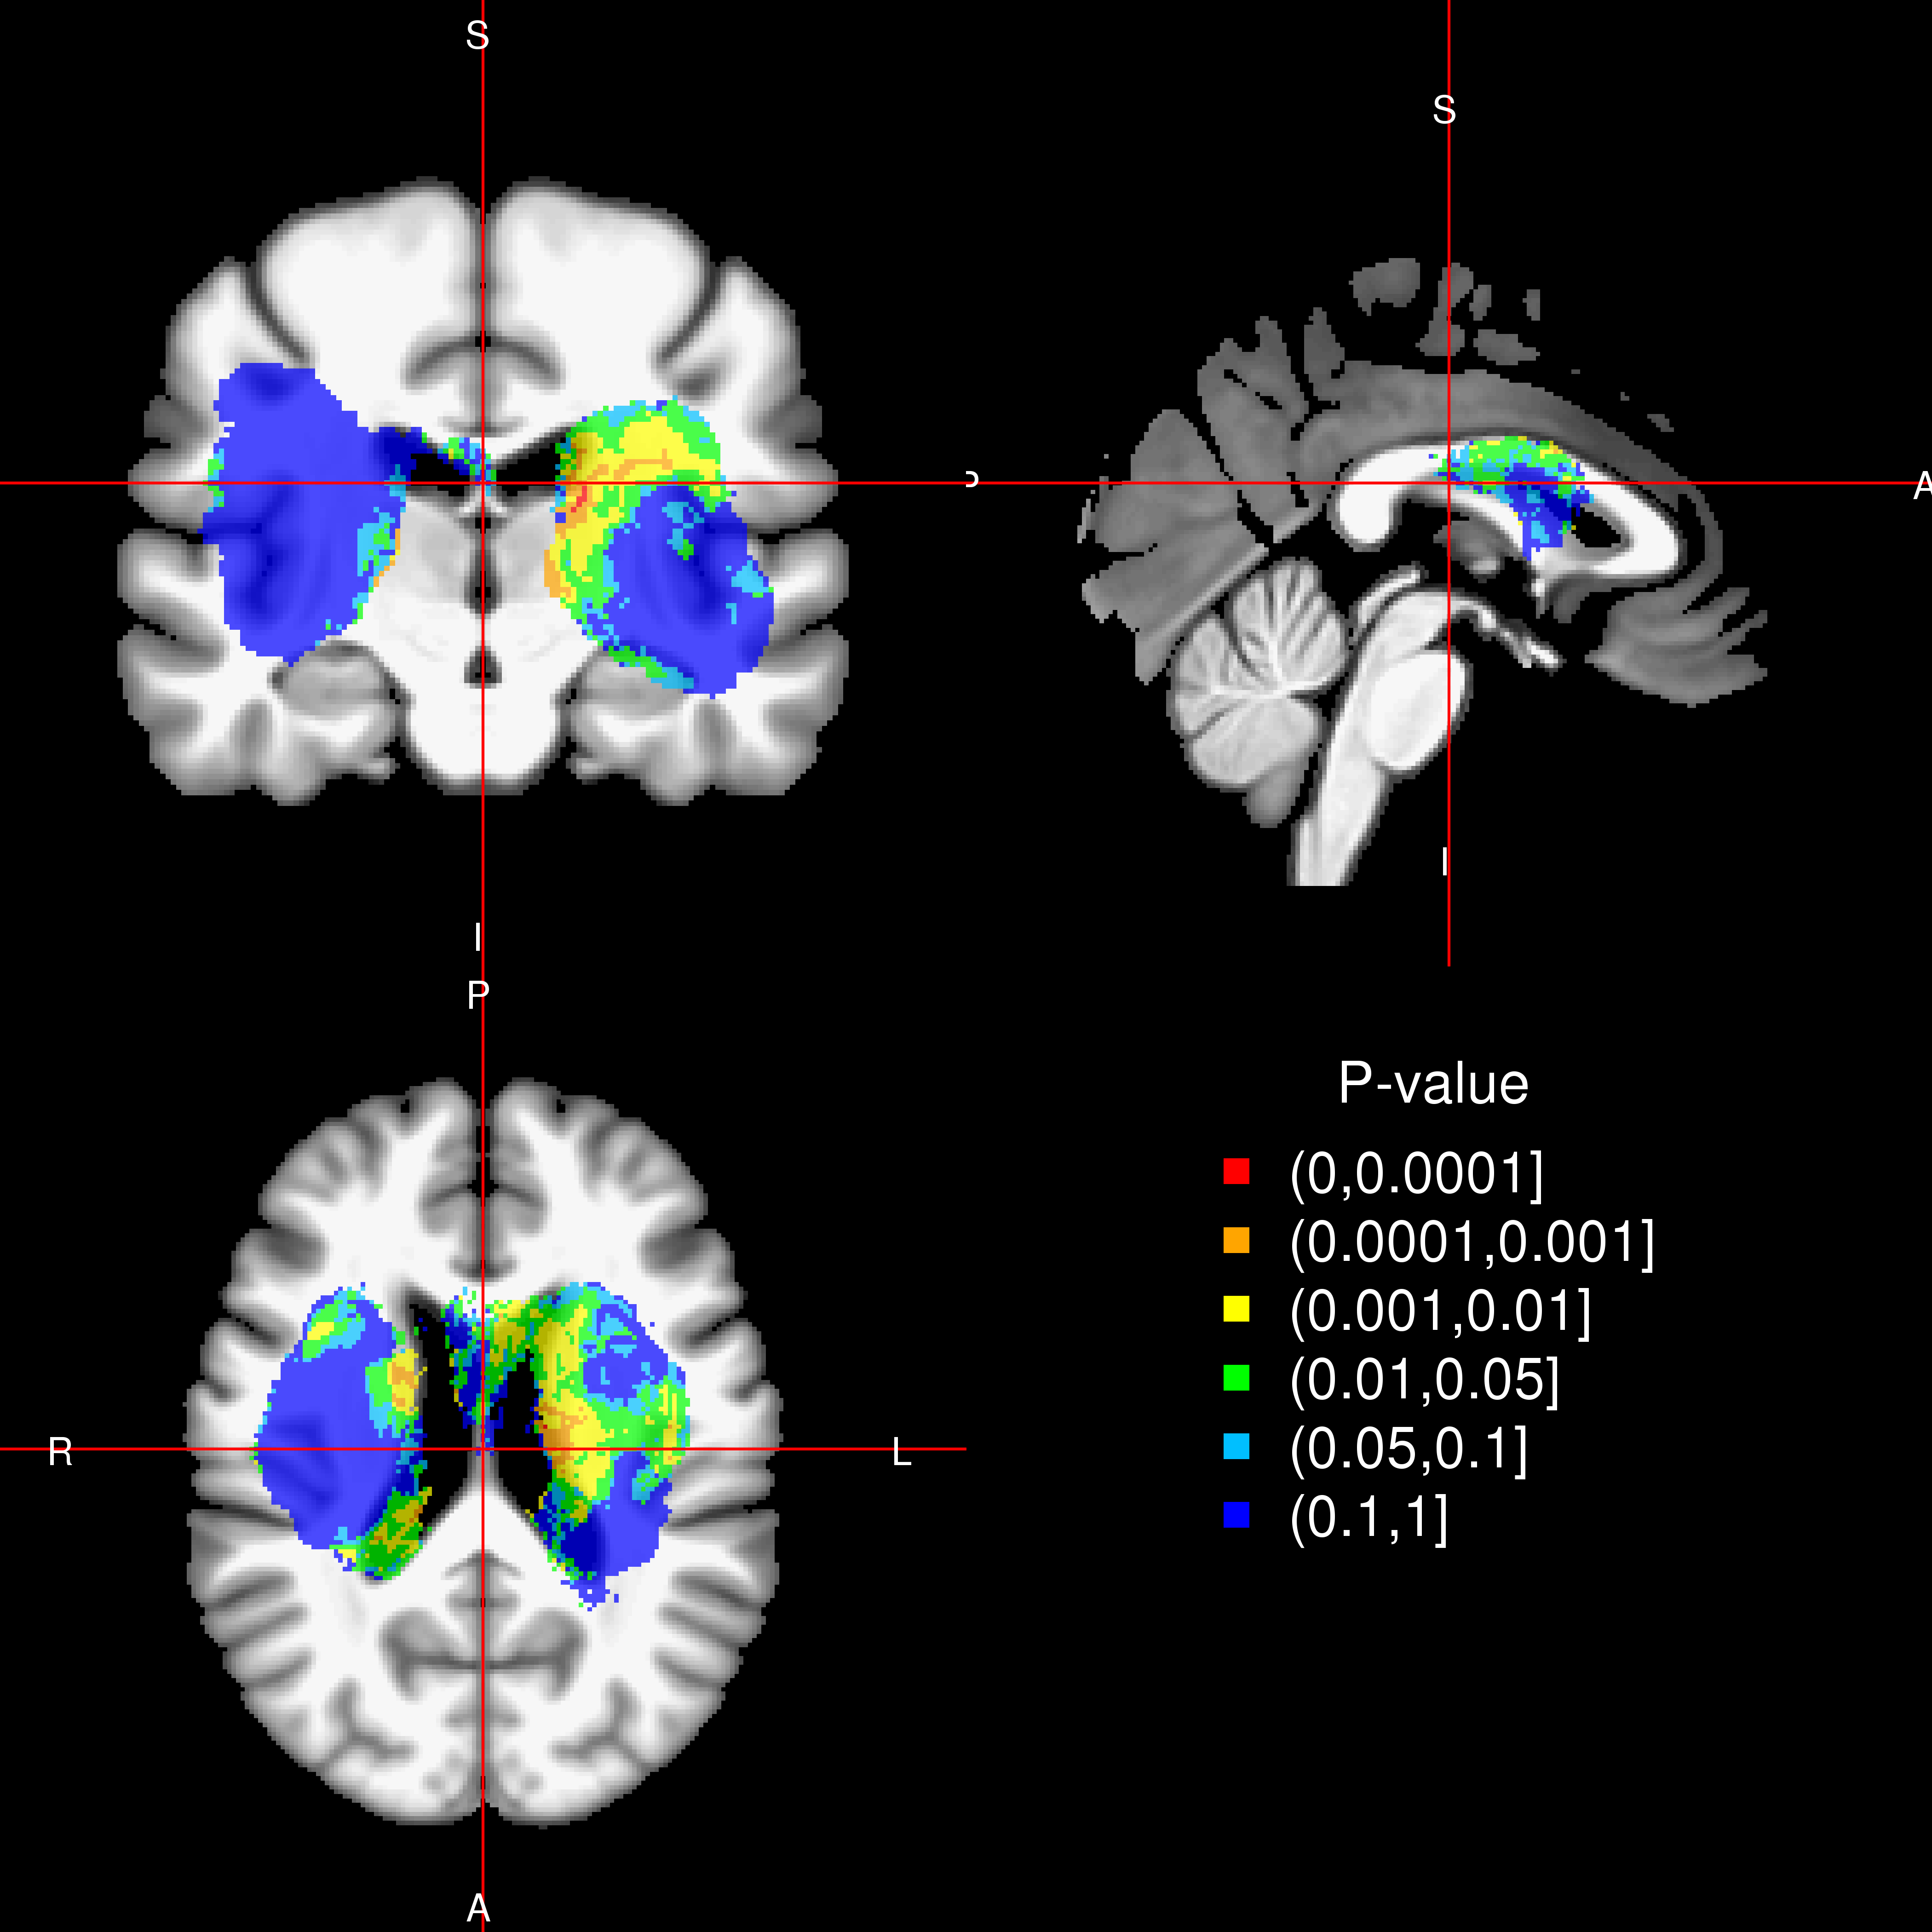
\includegraphics[width=.9\linewidth]{Regression_Map_heatcol1_t1.png}
\end{minipage}
~%
\begin{minipage}{.2\linewidth}
	{\color{color1} Figure 2:} Voxels with the smallest p-values seem to be near the ventricles.  No voxel survived a Bonferroni correction. \\	
	{\bf Take Home Message: We can do voxel-wise analyses with CT on scalar functional scores.}
\end{minipage}


\setcounter{figure}{2}

\vspace*{-.25cm}

%--References------------------------------------------------------------------

% \section{References}


%\renewcommand{\bibname}{\chapter{References}}
\section{References}
\setlength\bibitemsep{0pt}
\printbibliography[heading=none]\vspace*{-0.5cm}


{\small {\bf \small Funding: } The project described was supported by the  NIH grant RO1EB012547, NIA training grant T32AG000247, NINDS grants RO1NS060910 and RO1NS085211, and by NIMH grant RO1MH095836. JHU holds a use patent for intraventricular tissue plasminogen activator.}


\vfill
\columnbreak

\section{Creating a 3D Histogram of ICH Prevalence}
\vspace*{-.5cm}

\begin{figure}[htbp]
 \begin{subfigure}[t]{0.4\linewidth} 
  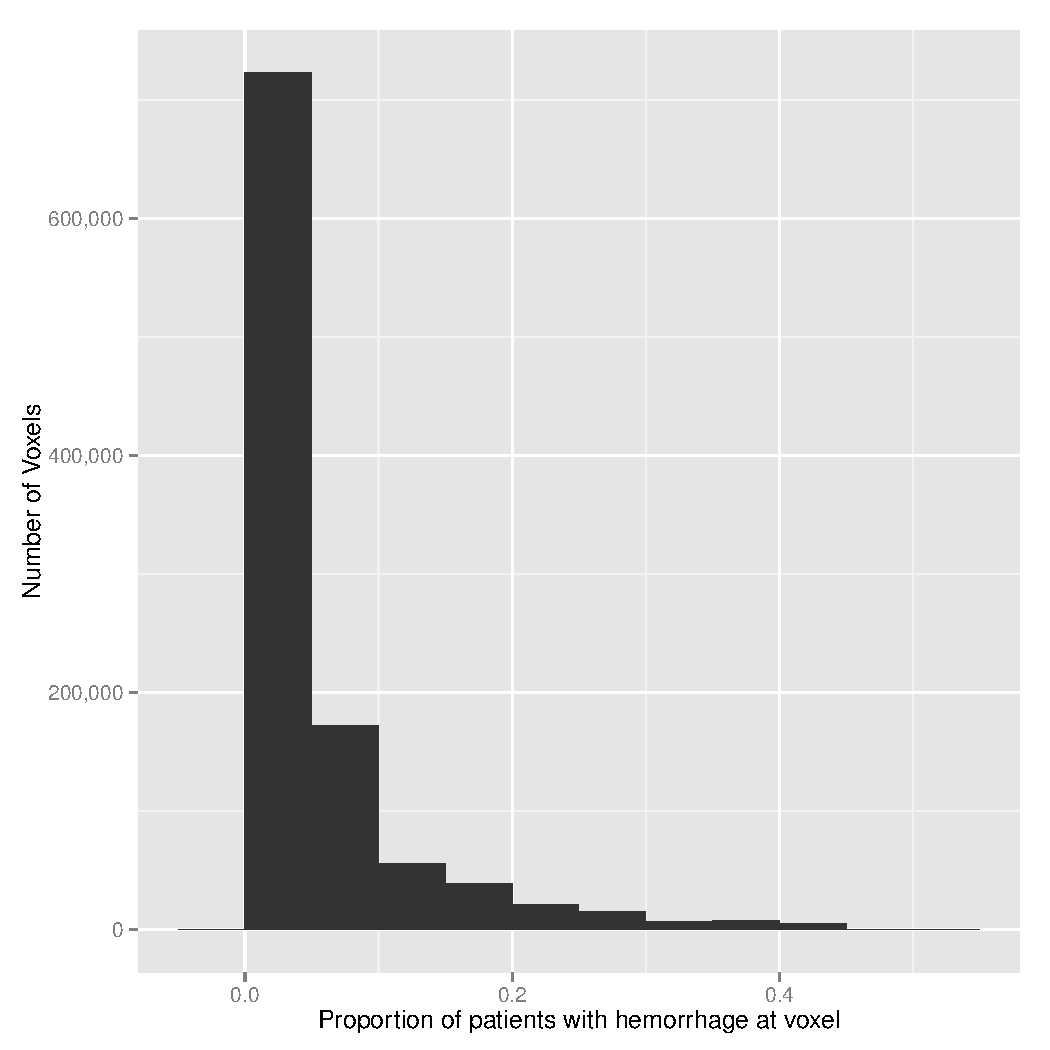
\includegraphics[width=\linewidth]{reoriented_Binary_Sum_Image_histogram.pdf}
   \caption{\textbf{Distribution} of proportion of patients with hemorrhage. All voxels with 0 proportion are excluded.}
  \label{prop:hist}
  \end{subfigure}
 \;\begin{subfigure}[t]{.4\linewidth} 
    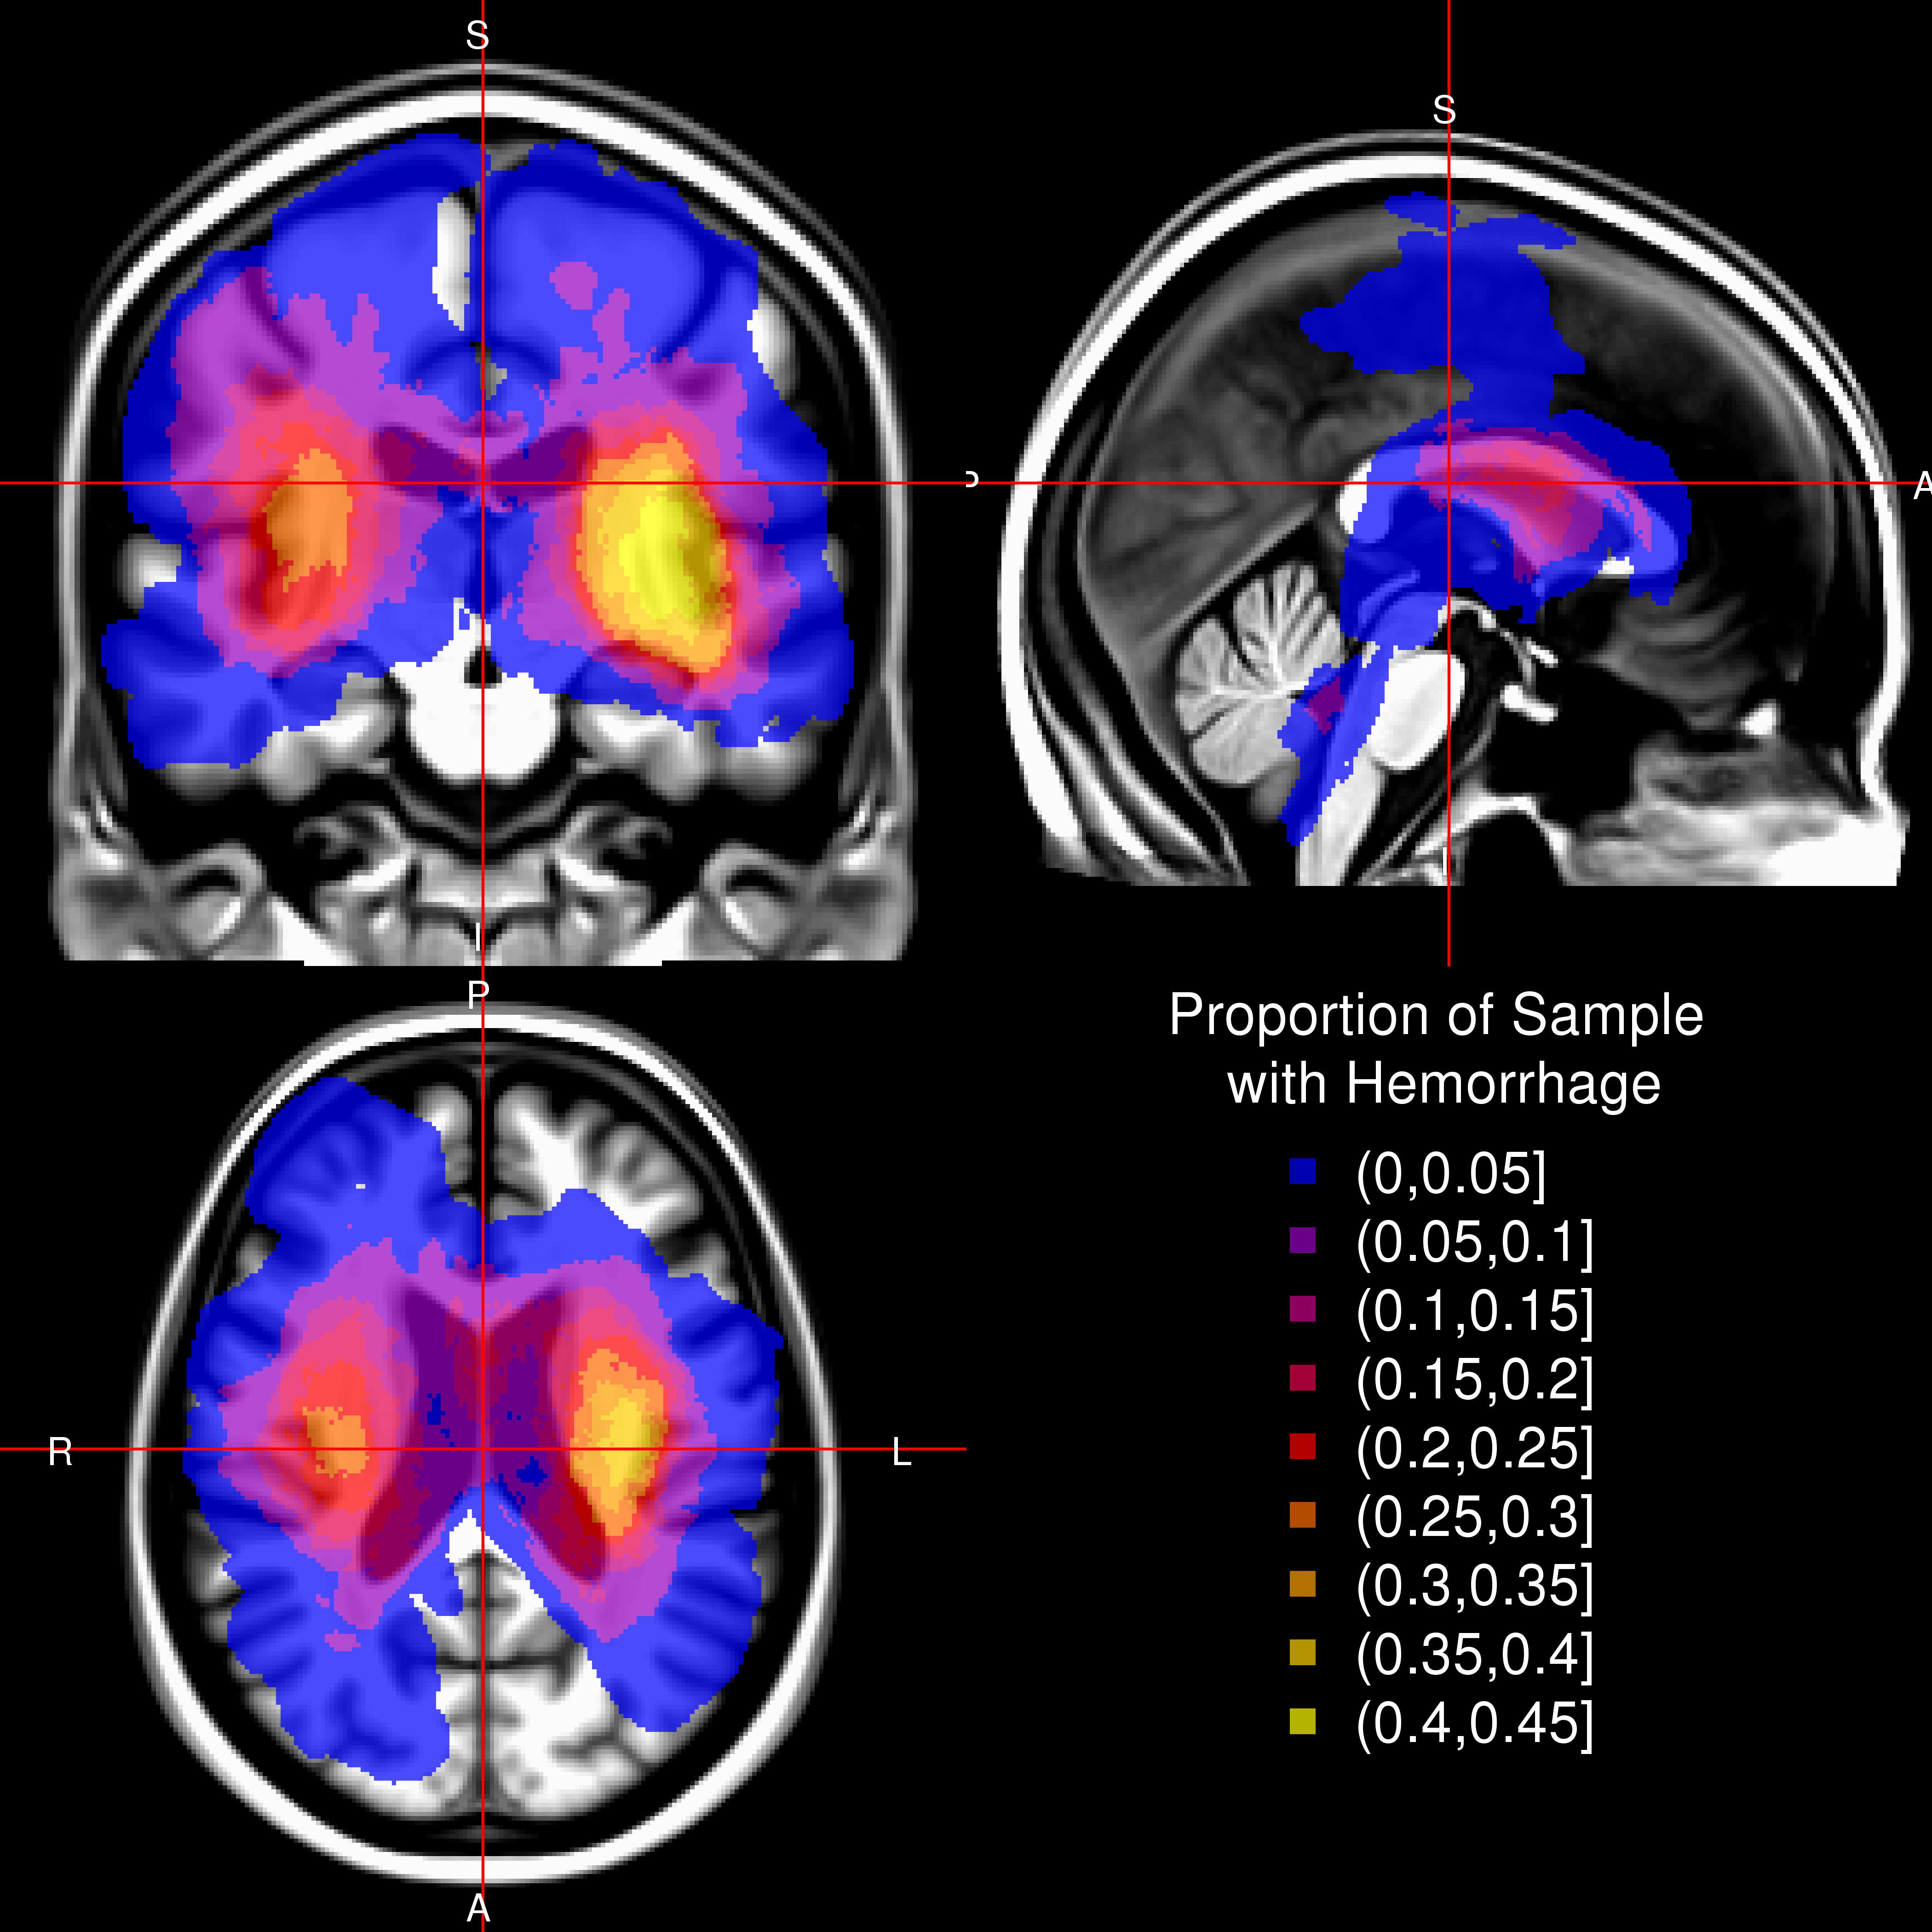
\includegraphics[width=\linewidth]{Figure4_Proportion.png}
   \caption{\textbf{Template brain (MRI T1)} with proportion of hemorrhage overlaid}
  \label{prop:img}
  \end{subfigure}
%   \begin{minipage}[b]{0.32\linewidth}
      \caption{Most voxels have a low prevalence (median: $3$\%), but some voxels ($V = 5685$) have prevalence $>40\%$.  In the spatial map, hotter colors (yellow) indicate more people had ICH at this location. Most ICH occurs in the middle of the brain, predominantly on the left.   {\bf Take Home Message: We can create population-level metrics/maps of ICH in this framework. }
  }
  \label{fig:StrokeHist}
%    \end{minipage}  
    \hfill
\end{figure}

\vspace*{-3cm}


\section{Region of Interest Analysis}

%\vspace*{-1cm}

We thresholded the p-values from model~\eqref{eq:vox} at $0.01$ (Figure~2) and created a ROI.  We used other thresholds, and the results were similar as below, but this threshold performed best.

\vspace*{-.5cm}
\begin{figure}[htbp]
\centering
  \begin{minipage}[t]{.29\linewidth}
\raisebox{-\height}{ 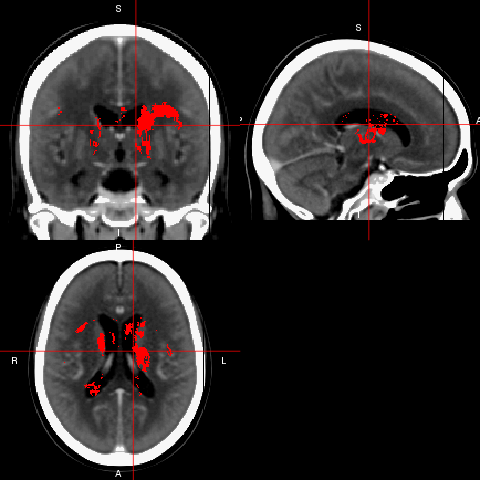
\includegraphics[width=\linewidth]{Top_19047_pvalues.png}}
\end{minipage}
~%
 \begin{minipage}[t]{0.65\linewidth}
 \caption[.]{The areas colored in red correspond to voxels with a p-value $< 0.01$ in the unadjusted model.  Of the voxels selected, we calculated a scan-level ROI coverage:\\
\begin{minipage}{\linewidth}
$$
\text{Coverage} = \frac{\text{\# Voxels classified ICH in ROI}}{\text{\# Voxels in ROI}}
$$
\vspace*{.5cm}

\end{minipage}
%\vspace{3cm}

\begin{minipage}{\linewidth}

This coverage is then put into the following patient-level model:
\begin{eqnarray}
{\rm NIHSS}_i&=&\beta_0+\beta_1 {\rm Coverage}_i +\beta_2 \text{Age}_i + \beta_3 \text{Sex}_i + \beta_2 \text{Total ICH Volume}_i  + \varepsilon_{i},\;\;\; \varepsilon_{i} \sim N\left(0, \sigma^2\right)\\
{\rm NIHSS}_i&=&\beta_0+\beta_{1j} {\rm Location}_{ij}+\beta_2 \text{Age}_i + \beta_3 \text{Sex}_i + \beta_2 \text{Total ICH Volume}_i  + \varepsilon_{i},\;\;\; \varepsilon_{i} \sim N\left(0, \sigma^2\right)
\end{eqnarray}
where ${\rm Location}_{ij}$ is an indicator that the ICH for patient $i$ was classified as location $j$, i.e. putamen or caudate.  
\vspace*{.5cm}

% latex table generated in R 3.0.2 by xtable 1.7-3 package
% Wed Jun 11 14:12:53 2014
\begin{table}[H]
\centering
\begin{tabular}{rr|cccc}
  \hline
{\bf Model} & {\bf P-value} & {\bf Adjusted R$^2$} & {\bf R$^2$} & {\bf AIC} & {\bf RMSE} \\ 
  \hline
Reader-Assessed ICH Location &  & 0.129 & 0.178 & 18.60 & 8.116 \\ 
  HPR Coverage & .0100 & 0.254 & 0.282 & 0.00 & 7.511 \\ 
   \hline
\end{tabular}
\caption{Table of model-fit measures for NIHSS score model: reader-based location vs. CT voxel-based HPR coverage.} 
\label{t:nihss}
\end{table}

{\bf Take Home Message: CT-level location information may be a better predictor than reader-assessed.}
\end{minipage}
}
  \label{f:roi} 
\end{minipage}  
\end{figure}





\section{Conclusions}
\vspace*{-0.5cm}
\begin{itemize}
%\item CT has different issues in analysis compared to magnetic resonance imaging (MRI), but MRI-based tools can be used in CT analysis.
\item Registration to a template allows for summaries of population of patients with ICH previously not available, with potentially more information.  
\item We can also do similar voxel-wise analyses as seen in the MRI literature with CT imaging.
\item CT-scan-level information of location better predicts NIHSS score better than reader-assessed categorization.
\end{itemize}

\section{Limitations}
\vspace*{-0.5cm}

We acknowledge the coverage has information about the outcome by the way the ROI was created.  This analysis is more exploratory and proof of concept than inferential.  We plan to do cross-validation as well as test the ROI performance in an independent set of individuals.  The population has exclusion criteria which may limit generalizability and are from a clinical trial population. 


%==============================================================================
%==End of content==============================================================
%==============================================================================


%--End of references-----------------------------------------------------------

\end{multicols}

%==============================================================================
\end{frame}
\end{document}
